\documentclass[a4,13pt]{extarticle}
\usepackage[utf8]{inputenc}
\usepackage[margin=2cm]{geometry}
\usepackage{amsmath}
\usepackage{graphicx}
\usepackage{algorithm}
\usepackage{algorithmicx}
\usepackage[]{algpseudocode}
\usepackage{hyperref}
\usepackage{color}
\usepackage{mathtools}
\usepackage{listings}
\DeclarePairedDelimiter\ceil{\lceil}{\rceil}
\DeclarePairedDelimiter\floor{\lfloor}{\rfloor}

\definecolor{blue}{rgb}{0,0,0.5}
\newenvironment{Solution}{\color{blue}\textbf{Solution:}}{}

\lstset{frame=tb,
  language=C,
  aboveskip=3mm,
  belowskip=3mm,
  showstringspaces=false,
  columns=flexible,
  basicstyle={\small\ttfamily},
  numbers=none,
  numberstyle=\tiny\color{gray},
  keywordstyle=\color{blue},
  commentstyle=\color{dkgreen},
  stringstyle=\color{mauve},
  breaklines=true,
  breakatwhitespace=true,
  tabsize=4
}

\title{COMP3506 Homework 1}
\author{Weighting: 15\%}
\date{Due date: 21st August 2020, 11:55 pm}

\begin{document}

\maketitle
\if 0
\section*{Overview}
This purpose of this assignment is for you to become familiar with understanding the main concepts and notation of asymptotic analysis of algorithms, to gain practice writing simple mathematical proofs, to learn how to read and write pseudocode algorithms, and to practice using binary search and writing and analysing recursive algorithms.

\section*{Marks}
This assignment is worth 15\% of your total grade. COMP3506 students will be marked on questions 1 to 4 out of \textbf{50 marks}. COMP7505 are required to additionally do question 5 and will be marked out of \textbf{60 marks}.\\\\
Partial marks \textit{may} be awarded for partially correct answers and answers lacking justification where it is required.

\section*{Submission Instructions}
\begin{itemize}
	\item Your answers to the written questions should be submitted as a file called \textbf{A1-[Your Student Number Here].pdf} via the \texttt{Homework 1 - Written} submission. Do not include your full name in your pdf submission.
	\item \textbf{Hand-written answers will not be marked.} If you are comfortable with the \LaTeX\  typesetting
	      system, it is strongly recommended that you write your answers using it, however it is not a requirement.
	\item Your solution to Q3a will be submitted via Gradescope to the \texttt{Homework 1 - Q3 Programming} submission. You should only submit your completed \texttt{ArrayCartesianPlane.java} file. No marks will be awarded for non-compiling submissions, or submissions which import non-supported 3rd party libraries. You should follow all constraints laid out in question 3 or risk losing marks for the question.
\end{itemize}

\section*{Late Submissions and Extensions}
Late submissions will not be accepted. It is your responsibility to ensure you have submitted your
work well in advance of the deadline (taking into account the possibility of computer, internet, or Gradescope
issues). You are allowed to submit multiple times, and only the latest submission before the deadline will be marked. See the ECP for information about extensions.
\section*{Academic Misconduct}
This assignment is an individual assignment. Posting questions or copying answers from the internet is considered cheating, as is sharing your answers with classmates. All your work (including code) will be analysed by sophisticated plagiarism detection software. \\\\
Students are reminded of the University’s policy on student misconduct, including plagiarism. See
the course profile and the School web page:
\url{http://www.itee.uq.edu.au/itee-student-misconduct-including-plagiarism}.\\

\newpage 

\fi 
\section*{Questions}

\begin{enumerate}
	\item   
	      Consider the following algorithm, \textsc{CoolAlgorithm}, which takes a \textbf{positive} integer $n$ and outputs another integer. 
	      Recall that `$\&$' indicates the bitwise AND operation and `$a >> b$' indicates the binary representation of $a$ shifted to the right $b$ times.
	      	      
	      \begin{algorithm}
	      	\begin{algorithmic}[1]
	      		\Procedure{CoolAlgorithm}{int n}
	      		\State $sum \gets 0$
	      		\If {$n$ \% $2 == 0$}
	      		\For{$i=0$ to $n$} 
	      		\For {$j=i$ to $n^2$}
	      		\State $sum \gets sum + i + j$ 
	      		\EndFor 
	      		\EndFor
	      		\Else
	      		\While{$n > 0$}
	      		\State $sum \gets sum$ + $(n$ \& $1)$
	      		\State $n \gets (n >> 1)$
	      		\EndWhile
	      		\EndIf
	      		\State \textbf{return} $sum$
	      		\EndProcedure
	      	\end{algorithmic}
	      \end{algorithm}
	      	          
	      Note that the runtime of the above algorithm depends not only on the size of the input $n$, but also on a numerical property of $n$. 
	      For all of the following questions, you must assume that $n$ is a positive integer.
	      	      
	      \begin{enumerate}
	      	\item (3 marks) Represent the running time (i.e. the number of primitive operations) of the algorithm 
	      	      when the input $n$ is \textbf{odd}, as a mathematical function called $T_{\text{odd}}(n)$. State all assumptions made and explain all your reasoning.
	      	      
	      	      \begin{Solution}
For $n$ odd, let us count the number of primitive operations.

Line 2 presents a single operation of assignment.

Line 3 presents a conditional checking if $n \% 2 == 0$. This is only true when $n$ is even, and hence the if block only contributes $1$ primitive operation, as it is never entered.

Then, observing the while loop, on each iteration, the while condition contributes $1$ primitive operation, and then we obtain an extra operation from the final while condition check when the while loop condition is false.

Within the while loop, on line $11$, we observe/assume $3$ primitive operations: the bitwise AND (assumed to be a single primitive operation), the addition, and the assignment of 'sum'.

On line $12$, there are $2$ primitive operations present: the right bitshift (this is assumed to be a single primitive operation), and the assignment.

Therefore, on each iteration of the while loop, $5$ operations occur within said loop body, and $1$ operation occurs to check if another iteration of the loop is to be conducted, hence $6$ primitive operations per successful while loop iteration.

Finally, Line 15 presents one more primitive operation to return the sum.

Therefore, $T_{\text{odd}}(n)=4+6\left(p(n)+1\right)$, where $p(n)$ denotes the number of loop iterations as a function of the input size.

Let us calculate $p(n)$.

We may assume that $n$ is represented as a binary number.

This implies that a single bit shift right would halve $n$ (via integer division).

Therefore, on each iteration, $n$ is halved, suggesting the number of iterations of the while loop is dependent on the nearest power of $2$ that $n$ is divisible by.

As a result, we may be model the number of iterations of the while loop by a $\floor{\log_2(n)}$ function, the floor function is implemented to ensure an integer amount of primitive operations.

Therefore, $T_{\text{odd}}(n)=4+6\left(\floor{\log_2(n)}+1\right)=10+6\floor{\log_2(n)}$.


	      	      \end{Solution}
	      	      	      	                  
	      	\item (2 marks) Find a function $g(n)$ such that $T_{\text{odd}}(n)\in O(g(n))$. 
	      	      Your $g(n)$ should be such that the Big-O bound is as tight as possible (e.g. no constants or lower order terms). 
	      	      Using the formal definition of Big-O, prove this bound and explain all your reasoning. 
	      	      	      	                  
	      	      (Hint: you need to find values of $c$ and $n_0$ to prove the Big-O bound you gave is valid).
	      	      
	      	       \begin{Solution}
Claim: $g(n)=\log_2(n)\implies T_{\text{odd}}(n)\in O(\log n)$.

By definition, an arbitrary function $f(n)$ is $O(g(n))$ if there exist positive constants $c$ and $n_0$ such that $f(n)\le cg(n)$ for all $n\geq n_0$.

To show that $T_{\text{odd}}(n)$ is $O(\log n)$, let us suppose that $T_{\text{odd}}(n)\le c\log_2(n)$, and attempt to find $c$ and $n_0$ values that uphold the proposed inequality.

First, observe that by the definition of the floor function, $10+6\floor{\log_2(n)}\le10 + 6\log_2(n)$.

Therefore, $10 + 6\log_2(n)\le c\log_2(n)$ implies $T_{\text{odd}}(n)\le c\log_2(n)$.

Clearly, $10 + 6\log_2(n)\le c\log_2(n)\implies10\le c\log_2(n)-6\log_2(n)$

\begin{center}
$\implies10\le\left(c-6\right)\log_2(n)$

$\implies\dfrac{10}{c-6}\le\log_2(n)$

$\implies2^{\frac{10}{c-6}}\le n$.
\end{center}

Then, if we pick say $c=8$, we see that $n\ge2^5=32$.

Therefore, if we let $n_0=32$ and $c=8$, we observe that there exist positive constants $c$ and $n_0$ such that $T_{\text{odd}}(n)\le c\log_2(n)$ for all $n\geq n_0$, implying that $T_{\text{odd}}(n)\in O(\log n)$.

Trivially, as $T_{\text{odd}}(n)$ is an unbounded, increasing function, there exists no constant that can act as an upper bound for $T_{\text{odd}}(n)$, for all $n$.

Thus, $O(\log n)$ is the tightest possible Big-O bound.
	      	      \end{Solution}
	      	      	      	                  
	      	\item (2 marks) Similarly, find the tightest Big-$\Omega$ bound of $T_{\text{odd}}(n)$ and use the formal definition of Big-$\Omega$ to prove the bound is correct. Does a Big-$\Theta$ bound for $T_{\text{odd}}(n)$ exist? If so, give it. If not, explain why it doesn't exist.
	      	
	      	\begin{Solution}
Claim: $g(n)=\log_2(n)\implies T_{\text{odd}}(n)\in\Omega(\log n)$.

By definition, an arbitrary function $f(n)$ is $\Omega(g(n))$ if there exist positive constants $c$ and $n_0$ such that $f(n)\ge cg(n)$ for all $n\geq n_0$.

To show that $T_{\text{odd}}(n)$ is $\Omega(\log n)$, let us suppose that $T_{\text{odd}}(n)\ge c\log_2(n)$, and attempt to find $c$ and $n_0$ values that uphold the proposed inequality.

First, observe that by the definition of the floor function, $10+6\floor{\log_2(n)}>9 + 6\log_2(n)$.

Therefore, $9 + 6\log_2(n)\ge c\log_2(n)\implies 10+6\floor{\log_2(n)}> c\log_2(n)$

If we let $c=6$, we observe the inequality holds for all positive $n$.

Thus, if we let $c=6$ and $n_0=1$, we obtain positive constants $c$ and $n_0$ such that $T_{\text{odd}}(n)\ge c\log_2(n)$, for all $n\ge n_0$.

Thus, $\Omega\left(\log n\right)$ is the tightest Big-$\Omega$ bound for $T_{\text{odd}}(n)$.

As shown in parts 1b and 1c, For all $n\ge 32, 6\log_2(n)\le T_{\text{odd}}(n)\le 8\log_2(n)$.

Thus, there exist positive constants $c_1=6$, $c_2=8$, $n_0=32$, such that for all $n\ge n_0$, $c_1\log_2(n)\le T_{\text{odd}}(n)\le c_2\log_2(n)$.

Hence, $T_{\text{odd}}(n)\in\Theta(\log n)$.
	      	\end{Solution}
	      	      	      	                  
	      	      	      	                  
	      	\item (3 marks) Represent the running time (as you did in part (a)) for the algorithm when the input $n$ is \textbf{even}, as a function called $T_{\text{even}}(n)$. State all assumptions made and explain all your reasoning. Also give a tight Big-O and Big-$\Omega$ bound on $T_{\text{even}}(n)$. You do \textbf{not} need to formally prove these bounds.
	      	
	      	\begin{Solution}
For $n$ even, let us count the number of primitive operations.

Line 2 presents a single operation of assignment.

Line 3 presents a conditional checking if $n \% 2 == 0$, this contributes $1$ primitive operation.

As the if statement is true for even $n$, we may enter it.

Entering the if statement, we observe a nested for loop. Let us call the number of operations obtained from said loop to be $p(n)$.

Finally, Line 15 presents one more primitive operation to return the sum.

Therefore, $T_{\text{even}}=3+p(n)$

Let us now obtain $p(n)$.

First, let us assume that '$i\gets0$ to $n$' implies that $i$ begins at $0$ and the loop runs as long as $i\le n$, as opposed to $i<n$. This same assumption is applied with regards to the inner loop (i.e. we consider the loop condition to be $j\le n^2$ instead of $j<n^2$).

First we count $1$ primitive operation for $i=0$.

Let $l$ denote the number of outer loop iterations (trivially, $l=n+1$).

Trivially, it may be observed that in any given for loop, there are $l$ loop increments, and $(l+1)$ loop condition checks.

Let $X$ be the number of primitive operations within the body of the outer loop.

Thus, $p(n)=1+l+l+1+X$

Let us now calculate $X$.

We apply a similar approach to the outer loop.

Trivially, we initialise $j=i$ once per iteration.

As there are $l$ iterations, we say that the operation '$j=i'$ occurs $l$ times.

Also, we assume that calculating $n^2$ only occurs once per outer loop iteration, rather than in each inner loop iteration (e.g. in C we may do something like this):

\begin{lstlisting}
for (int c = n^2, int j = i; j <= c; j++) {...}
\end{lstlisting}

Hence, we say that this operation will occur $l$ times as well.

Next, observe that on any given outer loop iteration $i$, by inspection we observe that the inner loop runs $(n^2-i+1)$ times.

Then, by the observation made earlier that the number of loop increments is equal to the number of loop iterations, this implies that there are $(n^2-i+1)$ loop increments for each outer loop iteration.

Now, observing line $6$, we see two addition operations and an assignment operation. Hence on each inner loop iteration, the inner loop body contributes $3$ primitive operations.

Furthermore, as the number of inner loop condition checks is $1$ greater than the number of inner loop iterations, we may count the extra loop condition check separately.

Thus, for any given iteration $i$ of the outer loop, there are $5\left(n^2-i+1\right)+1+1+1$ primitive operations within the inner loop body.

Then, as there are $l$ iterations of the outer loop, it is clear that $X=5\displaystyle\sum_{i=0}^n\left(n^2-i+1\right)+l+l+l$.

Let us simplify $X$.

\begin{center}
Observe that $\displaystyle\sum_{i=0}^n\left(n^2-i+1\right)=\displaystyle\sum_{i=0}^n\left(n^2+1-i\right)$

$=\displaystyle\sum_{i=0}^n\left(n^2+1\right)-\displaystyle\sum_{i=0}^ni$

$=\left(n+1\right)\left(n^2+1\right)-\dfrac{n\left(n+1\right)}2$

$=\dfrac{2\left(n+1\right)\left(n^2+1\right)-n\left(n+1\right)}2$

$=\dfrac{2n^3+n^2+n+2}2$

$\implies X=5\left(\dfrac{2n^3+n^2+n+2}2\right)+l+l+l$

$\implies p(n)=1+l+l+1+5\left(\dfrac{2n^3+n^2+n+2}2\right)+l+l+l$

$\implies p(n)=1+n+1+n+1+1+5\left(\dfrac{2n^3+n^2+n+2}2\right)+n+1+n+1+n+1$

$\implies p(n)=7+5n+5\left(\dfrac{2n^3+n^2+n+2}2\right)$

$\implies p(n)=7+5n+\dfrac{10n^3+5n^2+5n+10}2$

$\implies p(n)=7+5n+5n^3+\dfrac52n^2+\dfrac52n+5$

$\implies p(n)=5n^3+\dfrac52n^2+\dfrac{15}2n+12$

$\implies T_{\text{even}}=3+5n^3+\dfrac52n^2+\dfrac{15}2n+12$

\end{center}

Thus, $T_{\text{even}}=5n^3+\dfrac52n^2+\dfrac{15}2n+15$.

Now, calculating a tight Big-O bound for $T_{\text{even}}$:

Observe that $T_{\text{even}}$ is a polynomial of degree $3$.

Thus, as shown in class, $T_{\text{even}}\in O(n^3)$ by the first simplification rule of Big-O notation.

Now to obtain a tight Big-$\Omega$ bound, we claim that $T_{\text{even}}\in\Omega(n^3)$.

By definition, an arbitrary function $f(n)$ is $\Omega(g(n))$ if there exist positive constants $c$ and $n_0$ such that $f(n)\ge cg(n)$ for all $n\geq n_0$.

To show that $T_{\text{even}}(n)$ is $\Omega(n^3)$, let us suppose that $5n^3+\dfrac52n^2+\dfrac{15}2n+15\ge cn^3$, and attempt to find $c$ and $n_0$ values that uphold the proposed inequality.

Trivially, we may simply set $n_0=1$ and $c=1$ and we observe that $T_{\text{even}}(n)\in\Omega(n^3)$.
	      	\end{Solution}
	      	      	      	                  
	      	\item (2 marks) The running time for the algorithm has a best case and worst case, and which case occurs for a 
	      	      given input $n$ to the algorithm depends on the parity of $n$.
	      	      	      	                  
	      	      Give a Big-O bound on the \textbf{best case} running time of the algorithm, and a Big-$\Omega$ bound on 
	      	      the \textbf{worst case} running time of the algorithm (and state which parity of the input corresponds with which case).
	        \begin{Solution}
The best case running time of the algorithm occurs for odd $n$. This is because the tightest Big-O bound for $T_{\text{odd}}$ (i.e. $O(\log n)$), which represents an asymptotic upper bound for runtime, is always smaller than the tightest Big-O bound for $T_{\text{even}}$ (i.e. $O(n^3)$).

Therefore, the tightest Big-O bound for the best case running time of the algorithm is $O(\log n)$.

The worst case running time of the algorithm occurs for even $n$. This is because the tightest Big-$\Omega$ bound for $T_{\text{even}}$ (i.e. $O(n^3)$), which represents an asymptotic lower bound for runtime, is always greater than the tightest Big-$\Omega$ bound for $T_{\text{odd}}$ (i.e. $O(\log n)$).

Therefore, the tightest Big-$\Omega$ bound for the worst case running time of the algorithm is $O(n^3)$.
	      	\end{Solution}
	      	      	      	      
	      	      	      	                  
	      	\item (2 marks) We can represent the runtime of the entire algorithm, say $T(n)$, as
	      	      \begin{align*}
	      	      	T(n)=\begin{cases}
	      	      	T_{\text{even}}(n) & \text{if $n$ is even} \\
	      	      	T_{\text{odd}}(n)  & \text{if $n$ is odd}  \\
	      	      	\end{cases}
	      	      \end{align*}
	      	      Give a Big-$\Omega$ and Big-$O$ bound on $T(n)$ using your previous results. If a Big-$\Theta$ bound for the entire algorithm exists, describe it. If not, explain why it doesn’t exist.
	      	      
	      	\begin{Solution}
The tightest Big-$\Omega$ bound on $T(n)$, as it denotes an asymptotic lower bound for runtime, would be the tightest Big-$\Omega$ bound for the best case of $T(n)$.

This is when $n$ is odd, thus the tightest Big-$\Omega$ bound on $T(n)$ is equal to the tightest Big-$\Omega$ bound for $T_{\text{odd}}(n)$.

Therefore, $T(n)\in\Omega(\log n)$.

Similarly, the tightest Big-O bound on $T(n)$, as it denotes an asymptotic upper bound for runtime, would be the tightest Big-O bound for the worst case of $T(n)$.

This is when $n$ is even, thus the tightest Big-O bound on $T(n)$ is equal to the tightest Big-O bound for $T_{\text{even}}(n)$.

Therefore, $T(n)\in O(n^3)$.

It may be observed that this algorithm does not have a Big-$\Theta$ bound.

By definition, if there exist positive constants $c_1, c_2$, and $n_0$, such that $c_1g(n)\le T(n)\le c_2g(n)$ for all $n\geq n_0$, then $T(n)\in\Theta(g(n))$.

As $T(n)$ alternates for each integer $n$, and both $n^3$ and $\log n$ are unbounded, strictly increasing functions, there exists no function $g(n)$ that can bound $T(n)$ from both above and below via constants $c_1, c_2$, for all $n\geq n_0$, as for any such function $g(n)$ of choice, there will always exist some integers $n_1, n_2$ such that $T(n_1)\ge c_2g(n)$ and $T(n_2)\le c_1g(n)$.
	      	\end{Solution}
	      	      	      	                  
	      	\item (2 marks) Your classmate tells you that Big-O represents the worst case runtime of an algorithm, and similarly that 
	      	      Big-$\Omega$ represents the best case runtime. Is your classmate correct? Explain why/why not. 
	      	      Your answers for (e) and (f) \textit{may} be useful for answering this.
	      	      
	      	\begin{Solution}
No. Big-O/Big-$\Omega$ are not the same as worst/best case algorithmic runtime.

Big-O simply represents an asymptotic upper bound for any given function, and Big-$\Omega$ represents an asymptotic lower bound for any given function.

This does not necessarily imply that an upper bound of runtime in the worst case, is given by Big-O (similarly for Big-$\Omega$ and best case runtime). In fact, Big-O/$\Omega$ notation does not even need to represent any concept of runtime or algorithmic complexity at all.

As shown in part e, we can give a Big-O/$\Omega$ bound for any function. So we may provide a Big-O bound for the best case runtime of an algorithm, or a Big-$\Omega$ for the worse case runtime of an algorithm.
	      	\end{Solution}
	      	      	      	                  
	      	\item (1 mark) Prove that an algorithm runs in $\Theta (g(n))$ time if and only if its worst-case running time 
	      	      is $O(g(n))$ and its best-case running time is $\Omega(g(n))$.
	      	      
	      	\begin{Solution}
$\Rightarrow$

Suppose an algorithm runs in $\Theta(g(n))$ time. Let $f(n)$ denote a function that returns the maximum number of primitive operations completed by the algorithm, based on the input size.

Then, by definition, there exist $c_1, c_2,$ and $n_0$ such that $c_1g(n)\le f(n)\le c_2g(n)$, for all $n\ge n_0$.

By the definition of Big-O notation, if there exist positive constants $c$ and $n_1$ such that $f(n)\le cg(n)$ for all $n\geq n_1$, then $f(n)\in O(g(n))$.

Observe that by setting $c=c_2$, and $n_1=n_0$, we obtain said result.

Similarly, by the definition of Big-$\Omega$ notation, if there exist positive constants $\alpha$ and $n_2$ such that $f(n)\ge cg(n)$ for all $n\geq n_2$, then $f(n)\in O(g(n))$.

Again, if we set $\alpha=c_1$ and $n_2=n_0$, we obtain said result.

Hence, an algorithm running in $\Theta(g(n))$ time implies that its worst case running time is $O(g(n))$ and its best case running time is $\Omega(g(n))$.

$\Leftarrow$

Suppose an algorithm's worst case running time is $O(g(n))$ and its best case running time is $\Omega(g(n))$.

Then, by definition, there exist positive constants $c_1, n_1$ such that $f(n)\le c_1g(n)$ for all $n\geq n_1$.

Also, there exist positive constants $c_2, n_2$ such that $f(n)\ge c_2g(n)$ for all $n\geq n_2$.

Then, if we set $n_0=\max\{n_1,n_2\}$, we observe that there exist positive constants $c_1, c_2$ and $n_0$ such that $c_1g(n)\le f(n)\le c_2g(n)$ for all $n\geq n_0$.

By definition, this implies that $f(n)\in\Theta(g(n))$.

Hence, an algorithm having its worst case running time be $O(g(n))$ and its best case running time be $\Omega(g(n))$, implies that said algorithm runs in $\Theta(g(n))$.

This completes the proof.
	      	\end{Solution}
	      	      	      	                  
	      \end{enumerate}
	      	          
	      \newpage 
	      	
	\item 
	      \begin{enumerate}
	      	\item (4 marks) Devise a \textbf{recursive} algorithm that takes a sorted array $A$ of length $n$, containing distinct (not necessarily positive) integers, and determines whether or not there is a position $i$ (where $0\leq i < n$) such that $A[i] = i$.
	      	      \begin{itemize}
	      	      	\item Write your algorithm in pseudocode (as a procedure called $\textsc{FindPosition}$ that takes an input array $A$ and returns a boolean).
	      	      	\item Your algorithm should be as efficient as possible (in terms of time complexity) for full marks.
	      	      	\item You will not receive any marks for an iterative solution for this question. 
	      	      	\item You are permitted (and even encouraged) to write helper functions in your solution.
	      	      \end{itemize}
	      	      
	      	\begin{Solution}
	      \begin{algorithm}
	      	\begin{algorithmic}[1]
	      		\Procedure{FindPosition}{int[] A}
			\State\textbf{Input: }An array A of distinct, sorted integers.
			\State\textbf{Output: }Whether there exists a position $i$ such that $A[i]=i$, where $0\le i<length(A)$.
			\State\textbf{return} $CheckIndices(A, 0, length(A) - 1)$
	      		\EndProcedure
	      	\end{algorithmic}
	      \end{algorithm}

\begin{algorithm}
      	\begin{algorithmic}[1]
	      		\Procedure{CheckIndices}{int[] A, int leftPosition, int rightPosition}
			\State\textbf{Input: }An array A of distinct, sorted integers, the smallest index to search from, and the largest index to
			\State\,\,\,\,\,\,\,\,\,\,\,\,\,\,\,\,\,\,\,\,\,\,search to.
			\State\textbf{Output: }Whether there exists a position $i$ such that $A[i]=i$, where $0\le i<length(A)$.
      		\If {$rightPosition \geq leftPosition$}
			\State $midPoint \gets (leftPosition + rightPosition) / 2$
\If {$A[midPoint] = midPoint$}
\State \textbf{return} true
\ElsIf {$A[midPoint] < midPoint$}
\State \textbf{return} $CheckIndices(A, midPoint + 1, rightPosition)$
\Else
\State \textbf{return} $CheckIndices(A, leftPosition, midPoint - 1)$
	      		\EndIf
\EndIf
	      		\State \textbf{return} false
	      		\EndProcedure
	      	\end{algorithmic}
	      \end{algorithm}
	      	\end{Solution}
	      	
	      	\item (1 mark) Show and explain all the steps taken by your algorithm (e.g. show all the recursive calls, if conditions, etc) for the following input array: $[-1,0,2,3,10,11,23,24,102]$.
	      	
	      	\begin{Solution}
First, we are given the input of $A=[-1,0,2,3,10,11,23,24,102]$.

Thus, our algorithm will return the return value of the function call $CheckIndices(A, 0, length(A) - 1)$.

Trivially, $length(A)$ will return $9$, as there are $9$ elements in $A$.

Thus, our algorithm will return the return value of the function call $CheckIndices(A, 0, 8)$.

Observing this function call, we commence with $leftPosition\gets0$, and $rightPosition\gets8$.

We check \textbf{if} $rightPosition \geq leftPosition$, i.e. \textbf{if} $8\geq0$.

This is obviously true, so we enter the outer if block.

Then, we set $midPoint\gets(leftPosition + rightPosition) / 2$, i.e. $midPoint\gets(0+8)/2$

$\implies midPoint\gets4$.

Now, we check \textbf{if} $A[midPoint] = midPoint$, i.e. $A[4] = 4$.

As $A[4] = 10 > 4$, we do not enter the if block, nor the else if block (which checks \textbf{if} $A[midPoint] < midPoint$).

Hence, we enter the else block.

Here, we return the return value of the function call $CheckIndices(A, leftPosition, midPoint - 1)$.

i.e. We return the return value of the function call $CheckIndices(A, 0, 3)$.

Hence, the process described above repeats.

$rightPosition=3$ is still greater than $leftPosition=0$, so we may enter the outer if block.

This time, $midPoint\gets(0+3)/2\implies midPoint\gets1$.

$A[1] = 0 < 1\implies$ we enter the else if block.

As a result, we return the return value of the function call $CheckIndices(A, midPoint + 1, rightPosition)$.

i.e. We return the return value of the function call $CheckIndices(A, 2, 3)$.

Once more, the process described above repeats.

$rightPosition=3$ is still greater than $leftPosition=2$, so we may enter the outer if block.

This time, $midPoint\gets(2+3)/2\implies midPoint\gets2$.

$A[2] = 2\implies$ we enter the inner if block.

Thus, we return true. This return value propagates back to the original function call, resulting in the algorithm returning true.
	      	\end{Solution}
	      	      	      	                  
	      	\item (3 marks) Express the worst-case running time of your algorithm as a mathematical recurrence, $T(n)$, and explain your reasoning. 
	      	      Then calculate a Big-O (or Big-$\Theta$) bound for this recurrence and show all working used to find this bound 
	      	      (Note: using the Master Theorem below for this question will not give you any marks for this question).
	      	      
	      	      
	        \begin{Solution}
Let $n=length(A)$.

Observe that $n=0\implies length(A)-1=n-1=-1$.

Thus, on the first call to $CheckIndices(A, 0, -1)$, we have $rightPosition<leftPosition$.

As a result, the outer if block is never entered, and 'false' is returned immediately.

Hence, when $n=0$, a constant of $3$ primitive operations occur.

In the general case, observe that on any given recursive step, the region of the array searched is halved in size.

Hence, we may express $T(n)$ as follows:

\begin{center}
$T(n)=\begin{cases}O(1), & n=0, \\ T\left(\dfrac{n}2\right)+O(1), & n>0.\end{cases}$ 
\end{center}

To calculate a Big-O bound for $T(n)$, let us first make the following observation.

\begin{center}
For $n>0$,

$T(n)=O(1)+T\left(\dfrac{n}2\right)$

$=O(1)+O(1)+T\left(\dfrac{n}4\right)$

$=O(1)+O(1)+O(1)+T\left(\dfrac{n}8\right)$

\dots
\end{center}

Observe that as $n$ halves on each call, there must be at most $\floor{\log_2(n)}$ recursive calls in total.

Then, in the end we will simply have at most $\floor{\log_2(n)}$ calls of runtime complexity $O(1)$ in the worst case.

Thus, we may say that $T(n)\in O(\log n)$.
	      	\end{Solution}
	      	
	      	\item The master theorem is a powerful theorem that can be used to quickly calculate a tight asymptotic bound on a mathematical recurrence. A simplified version is stated as follows: Let $T(n)$ be a non-negative function that satisfies
	      	      \begin{align*}
	      	      	T(n)                              & = \begin{cases}    
	      	      	aT\left(\frac{n}{b}\right) + g(n) & \text{for $n > k$} \\
	      	      	c                                 & \text{for $n=k$}   
	      	      	\end{cases}
	      	      	\intertext{where $k$ is a non-negative integer, $a\geq 1$, $b\geq 2$, $c > 0$, and $g(n)\in \Theta(n^d)$ for $d\geq 0$. Then,}
	      	      	T(n)                              & \in \begin{cases}  
	      	      	\Theta(n^d)                       & \text{if $a<b^d$}  \\
	      	      	\Theta(n^d\log n)                 & \text{if $a=b^d$}  \\
	      	      	\Theta(n^{\log_b a})              & \text{if $a>b^d$}  
	      	      	\end{cases}
	      	      \end{align*}
	      	      \begin{enumerate}
	      	      	\item (1 mark) Use the master theorem, as stated above, to find a Big-$\Theta$ bound (and confirm your already found Big-O) for the recurrence you gave in (b). Show all your working.
	      	      	
	      	      	\begin{Solution}
Clearly, if we let

\begin{center}
$a=1$

$b=2$

$d=0$ $(\implies n^d=n^0=1)$

$k=0$

$g(n)=c=3\in O(1)\implies g(n)\in\Omega(1)\implies g(n)\in\Theta(1)$ (as per the result from 1h),

\end{center}

it is then clear that 

\begin{center}
$T(n) = \begin{cases}O(1), & n=0, \\\\ T\left(\dfrac{n}2\right)+O(1), & n>0.\end{cases}$
\end{center}

satisfies the conditions of the master theorem.

Then, $a=1=b^d=2^0\implies T(n)\in\Theta(n^0\log n)$.

i.e. $T(n)\in\Theta(\log n)$.
	      	        \end{Solution}
	      	
	      	      	\item (1 mark) Use the master theorem to find a Big-$\Theta$ bound for the recurrence defined by $$T(n)=5 \cdot T\left(\frac{n}{3}\right) + n^2 + 2n$$ and $T(1)=100$. Show all working.
	      	      	      	
	      	      	\begin{Solution}
We may rewrite $T(n)$ as follows:

\begin{center}
$T(n)= \begin{cases}5T\left(\dfrac{n}{3}\right) + n^2+2n, & \text{for $n > 1$}, \\100 & \text{for $n=1$}.\end{cases}$
\end{center}

Then, it is easy to observe that if we set

\begin{center}
$a=5$

$b=3$

$c=100$

$k=1$

$g(n)=n^2+2n\in O(n^2), \Omega(n^2)$ (as per simplification rules)

$\implies g(n)\in\Theta(n^2)$ (as per the result proved in 1h)

$\implies d=2$
\end{center}

then $a=5<b^d=3^2=9$.

Therefore, $T(n)\in\Theta(n^2)$.
	      	        \end{Solution}
	      	
	      	      	\item (1 mark) Use the master theorem to find a Big-$\Theta$ bound for the recurrence defined by $$T(n)=8 \cdot T\left(\frac{n}{4}\right) + 5n + 2\log n +\frac 1n $$ and $T(1)=1$. Show all working.
	      	      	
	      	      	\begin{Solution}
We may rewrite $T(n)$ as follows:

\begin{center}
$T(n)= \begin{cases}8T\left(\dfrac{n}{4}\right) + 5n + 2\log n +\dfrac 1n, & \text{for $n > 1$}, \\1 & \text{for $n=1$}.\end{cases}$
\end{center}

Set

\begin{center}
$a=8$

$b=4$

$c=1$

$k=1$

$g(n)=5n + 2\log n +\dfrac 1n$.
\end{center}

Then, let us attempt to find a Big-$\Theta$ bound for $g(n)$.

As shown in 1h, if we find the tightest Big-O and Big-$\Omega$ bounds for $g(n)$, and we observe that said bounds are equal, then this must be the tightest Big-$\Theta$ bound for $g(n)$.

Observe that $5n+2\log n+\dfrac1n\le6n$, for all $n\geq1$.

Thus, $g(n)\in O(n)$.

Also, observe that $5n+2\log n+\dfrac1n\geq4n$, for all $n\geq1$.

Thus, $g(n)\in\Omega(n)$.

Therefore, $g(n)\in\Theta(n)$ (as per the result proved in 1h)

$\implies d=1$.

Then, $a=8>b^d=4^1=4$.

Therefore, $T(n)\in\Theta(n^{\log_4(8)})$.

Observe that

\begin{center}
$\log_4(8)=\dfrac{\log_2(8)}{\log_2(4)}$

$=\dfrac{\log_2(2^3)}{\log_2(2^2)}$

$=\dfrac{3\log_2(2)}{2\log_2(2)}$

$=\dfrac32$
\end{center}

Therefore, $T(n)\in\Theta(n^\frac32)$.
	      	        \end{Solution}
	      	      \end{enumerate}
	      	      	      	                  
	      	\item (2 marks) Rewrite (in pseudocode) the algorithm you devised in part (a), but this time \textbf{iteratively}. 
	      	      Your algorithm should have the same runtime complexity of your recursive algorithm. Briefly explain how you determined the runtime complexity of your iterative solution.
	      	      
\begin{Solution}
\begin{algorithm}
      	\begin{algorithmic}[1]
	      		\Procedure{FindPosition}{int[] A}
\State\textbf{Input: }An array A of distinct, sorted integers.
			\State\textbf{Output: }Whether there exists a position $i$ such that $A[i]=i$, where $0\le i<length(A)$.
\State $leftPosition\gets0$
\State $rightPosition\gets length(A) - 1$
      		\While {$rightPosition \geq leftPosition$}
			\State $midPoint \gets (leftPosition + rightPosition) / 2$
\If {$A[midPoint] = midPoint$}
\State \textbf{return} true
\ElsIf {$A[midPoint] < midPoint$}
\State $leftPosition\gets midPoint + 1$
\Else
\State $rightPosition\gets midPoint - 1$
	      		\EndIf
\EndWhile
	      		\State \textbf{return} false
	      		\EndProcedure
	      	\end{algorithmic}
	      \end{algorithm}

Let us represent runtime complexity in terms of the tightest Big-O bound in the worst case.

Trivially, all primitive operations before, after, and within the loop are of constant time, as the only operations present are assignment of integers, conditionals between integers, addition of integers, and indexing.

Hence, the number of loop iterations in the worse case will dictate the tightest Big-O bound.

Observe that on any given iteration of the loop, either leftPosition, or rightPosition is changed to $1$ greater than, or less than midPoint respectively.

This effectively halves the region of the array $A$ being searched.

Hence, in the worst case, $\floor{\log_2(n)}$ loop iterations occur.

Thus, the worst case run time is bounded by $O(\log n)$.
	      	\end{Solution}
	      	      	      	                  
	      	\item (2 marks) While both your algorithms have the same runtime complexity, one of them will usually be faster in practice 
	      	      (especially with large inputs) when implemented in a procedural programming language (such as Java, Python or C). 
	      	      Explain which version of the algorithm you would implement in Java - and why - if speed was the most important factor to you. 
	      	      You may need to do external research on how Java method calls work in order to answer this question in full detail. 
	      	      Cite any sources you used to come up with your answer.\\
	      	      	      	                  
	      	      In addition, explain and compare the space complexity of your both your recursive solution 
	      	      and your iterative solution (also assuming execution in a Java-like language).
	      	      
	        \begin{Solution}
If speed was the most important factor, I would pick the iterative solution.

On each recursive method call, local variables are to be stored on the stack. This significantly increases the number of primitive operations performed as although the iterative solution would require the same number of loop iterations as the recursive solution would method calls, fewer instructions are required to iterate a loop compared to handling the stack frame (Reference: CSSE2010).

Regarding space complexity, recursive solutions are significantly more expensive for the same reasons: each recursive call requires the previous call's local variables to be stored on the stack.

Hence, for large $n$, $\floor{\log_2(n)}$ function calls worth of local variables would need to be stored on the stack, as opposed to the iterative case, where only $1$ function call is required.

Observing each individual function call, for both algorithms, a linear space complexity is observed.

Let $n=length(A)$.

Clearly, when larger-sized arrays are input into either algorithm, the space complexity will grow linearly.

All other local variables do not require more memory based on the size of A (unless $n$ grows larger than the size of an integer in whichever language the algorithm is implemented in), hence maintain constant space complexity.

As a result, the iterative solution has a tight $O(n)$ upper bound for space complexity, whereas, due to the $\floor{\log_2(n)}$ function calls in the recursive solution, the recursive solution has a tight $O(n\log n)$ upper bound for space complexity.
	      	\end{Solution}
	      \end{enumerate}
	      	              
	      \newpage 
	      	          
	\item
	      In the support files for this homework on Blackboard, we have provided an interface called \texttt{CartesianPlane} which describes a 2D plane which can hold elements at $(x,y)$ coordinator pairs, where $x$ and $y$ could potentially be negative. 
	      \begin{enumerate}
	      	\item (5 marks) In the file \texttt{ArrayCartesianPlane.java}, you should implement the methods in the interface \texttt{CartesianPlane} using a multidimensional array as the underlying data structure.
	      	      	      	                      
	      	      Before starting, ensure you read and understand the following:
	      	      \begin{itemize}
	      	      		      	      	
	      	      	\item Your solution will be marked with an automated test suite. 
	      	      	      	      	      	                          
	      	      	\item Your code will be compiled using Java 11.
	      	      	      	      	      	                          
	      	      	\item Marks may be deducted for poor coding style. You should follow the CSSE2002 style guide, which can be found on Blackboard.
	      	      	      	      	      	                          
	      	      	\item  A sample test suite has been provided in \texttt{CartesianPlaneTest.java}. 
	      	      	      This test suite is not comprehensive and there is no guarantee that passing these will ensure passing 
	      	      	      the tests used during marking. It is recommended, but not required, that you write your own tests for your solution.
	      	      	      	      	    
	      	      	      	   	                          
	      	      	\item You may not use anything from the Java Collections Framework (e.g. ArrayLists or HashMaps). If unsure about whether you can use a certain import, ask on Piazza.
	      	      	                               
	      	      	\item Do not add or use any static member variables. Do not add any \textbf{public} variables or methods.
	      	      	\item Do not modify the interface (or \texttt{CartesianPlane.java} at all), or any method signatures in your implementation.
	      	      \end{itemize}
	      	      	      	                      
	      	\item (1 mark) State (using Big-O notation) the memory complexity of your implementation, 
	      	      ensuring you define all variables you use. Briefly explain how you came up with this bound.
	      	      
	        \begin{Solution}
The member variables used in my implementation are:

\begin{itemize}
	      	      	\item \texttt{this.grid} - a 2D array with dimensions $m\times n$
	      	      	\item \texttt{this.minimumX} - The minimum x co-ordinate in which an item can be stored at
	      	      	\item \texttt{this.minimumY} - The minimum y co-ordinate in which an item can be stored at
	      	      	\item \texttt{this.maximumX} - The maximum x co-ordinate in which an item can be stored at
	      	      	\item \texttt{this.maximumY} - The maximum y co-ordinate in which an item can be stored at
	      	      \end{itemize}

In addition to the member variables, the resize() method presents a temporary local variable 'newGrid', whose reference is assigned to this.grid.

In the worst case, this resize()d grid is larger than the original this.grid.

Let 'newGrid' have dimensions $x\times y$, where $x\geq m$, and/or $y\geq n$.

Then, my implementation's memory complexity is bounded by $O(xy)$ (i.e. quadratic complexity).

It is to be noted that other variables such as method parameters, as well as the member variables denoting the maximum and minimum $x$ and $y$ co-ordinates, require a constant amount of memory and as such, can be disregarded by the simplification rules of Big-O notation.
	      	\end{Solution}
	      	      	      	                      
	      	\item (1 mark) Using the bound found above, evaluate the overall memory efficiency of your implementation. 
	      	      You should especially consider the case where your plane is very large but has very few elements.
	      	
	      	\begin{Solution}
My implementation's memory complexity is fixed by its grid size, not by the amount of elements.

As a result, often a lot of space is wasted when there are more available positions to place elements than there are elements.

A remedy to this would be to use an implementation of the List interface, such as ArrayList, which allows for dynamic resizing.

Naturally, arrays offer better time complexity than List implementations, due to the allocation of contiguous memory, which allows for constant-time indexing.

However, from the perspective of memory efficiency alone, arrays offer absolutely no benefit.
	      	\end{Solution}
	      	      	      	                      
	      	\item (3 marks) State (using Big-O notation) the time complexity of the following methods:
	      	      	      	                      
	      	      \begin{itemize}
	      	      	\item \texttt{add}
	      	      	\item \texttt{get}
	      	      	\item \texttt{remove}
	      	      	\item \texttt{resize}
	      	      	\item \texttt{clear}
	      	      \end{itemize}
	      	      	      	                      
	      	      Ensure you define all variables used in your bounds, and briefly explain how you came up with the bounds. 
	      	      State any assumptions you made in determining your answers. You should simplify your bounds as much as possible.
	      	      
	      	\begin{Solution}
For \texttt{add}, as the number of primitive operations has no dependency on the size of \texttt{this.grid}, nor its input parameters, this method has time complexity $O(1)$, as it simply performs a conditional check, an assignment of a single position in \texttt{this.grid}, and potentially throws an exception. This is also true for \texttt{get} and \texttt{remove}, both of which also have $O(1)$ time complexity for the same reasons.

Regarding \texttt{clear}, if we let $m$ denote the number of 1D arrays within \texttt{this.grid}, and $n$ denote the length of each 1D array, then we may say that \texttt{clear} is $O(mn)$ time. As although all that occurs is a single assignment, where \texttt{this.grid} is assigned a new 2D array of the same size, Java initialises empty array elements to \texttt{null}, and hence it must do so for $mn$ elements.

Finally, regarding \texttt{resize}, this is also is bounded by $O(mn)$ time (i.e. quadratic complexity).

This is because the body of the nested for loop runs $mn$ times (as it only indexes the original 2D array), and said body only contains constant-time operations such as array indexing, assignment, and exception handling.

Only conditionals, and assignment occurs outside the nested for loop, and hence these are also constant-time operations.
	      	\end{Solution}
	      \end{enumerate}
	      	              
	      	              
	      \newpage 
	      	
	\item  
	      The UQ water well company has marked out an $n\times n$ grid on a plot of land, in which their hydrologists know exactly 
	      one square has a suitable water source for a water well. They have access to a drill, which uses drill bits and can test one 
	      square at a time. Now, all they they need is a strategy to find this water source.
	      	         
	      Let the square containing the water source be $(s_x,s_y)$. After drilling in a square $(x,y)$, certain things can 
	      happen depending on where you drilled.
	      \begin{itemize}
	      	\item If $x > s_x$ or $y > s_y$, then the drill bit breaks and must be replaced.
	      	\item If $x=s_x$ or $y=s_y$, the hydrologists can determine which direction the water source is in.
	      \end{itemize}
	      	              
	      Note that both the above events can happen at the same time. Below is an example with $n=10$ and $(s_x, s_y)=(3, 4)$. 
	      The water source is marked with \textsf{\textbf{S}}. Drilling in a shaded square will break the drill bit, and drilling in 
	      a square with a triangle will reveal the direction.
	      \begin{center}
	      	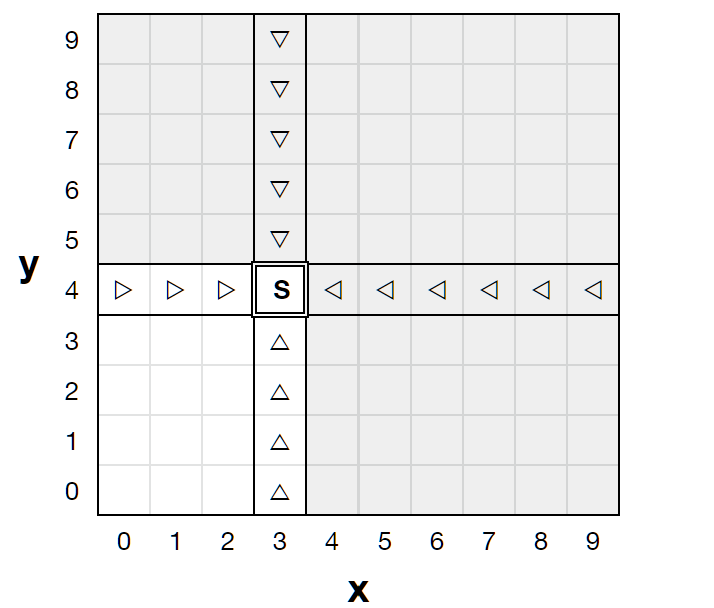
\includegraphics[width=0.4\textwidth]{a1q4new.png}
	      \end{center}
	      	              
	      \begin{enumerate} 
	      	\item (3 marks) The UQ water well company have decided to hire you - an algorithms expert - to devise a algorithm 
	      	      to find the water source as efficiently as possible. \\
	      	      	      	              
	      	      Describe (you may do this in words, but with sufficient detail) an algorithm to solve the problem of finding the water source, 
	      	      assuming you can break as many drill bits as you want. Provide a Big-O bound on the number of holes you need to drill to find 
	      	      it with your algorithm. Your algorithm should be as efficient as possible for full marks.\\\\
	      	      You may consult the hydrologists after any drill (and with a constant time complexity cost to do so) to see if 
	      	      the source is in the drilled row or column, and if so which direction the water source is in.\\\\
	      	      (Hint: A linear time algorithm is not efficient enough for full marks.)
	      	      
	      	\begin{Solution}
Let us implement an iterative algorithm that searches until $x=s_x$ and $y=s_y$.

Initially, we set $x\gets\dfrac{n}2$ and $y\gets\dfrac{n}2$ and drill.

Then, we consult the hydrologists to see if the source is in the drilled row or column.

If we have found both the correct row ($y$) and column ($x$), then we have found the water source and are finished.

If we have found either the correct row or the correct column (but not both, i.e. exclusive or), we maintain the same $x$ or $y$ value (whichever is correct), and then check which direction the water is in.

We the approach the direction of water by either doubling, or halving our current incorrect value.

For example, if the correct row is drilled (i.e. $y=s_y$), and the direction of the water source is left of the current $x$ (i.e. $x>s_x$), then we set $x\gets\dfrac{x}2$.

Other cases follow analogously.

If we find neither the correct row or column, we check if our drill bit has broken.

If it has, we set $x\gets\dfrac{x}2$, and $y\gets\dfrac{y}2$.

Otherwise, we set $x\gets2x$, and $y\gets2y$.

Clearly, as we halve the search area on each iteration, the number of holes needed to be drilled to find the water source is bounded by $O(\log n)$.

i.e. We are simply applying binary searches to both the $x$ and $y$ co-ordinates.
	      	\end{Solution}
	      	      	      	              
	      	\item 
	      	      (5 marks) The company, impressed with the drilling efficiency of your algorithm, assigns you to another $n \times n$ grid, 
	      	      which also has a water source you need to help find. However, due to budget cuts, this time you can only break $2$ drill 
	      	      bits (at most) before finding the source. (Note that you are able to use a $3$rd drill bit, but are not allowed to ever break it).
	      	      	      	              
	      	      Write \textbf{pseudocode} for an algorithm to find the source while breaking at most $2$ drill bits, and give a tight Big-O 
	      	      bound on the number of squares drilled (in the worst case). If you use external function calls (e.g. to consult the hydrologist, 
	      	      or to see if the cell you drilled is the source) you should define these, their parameters, and their return values. \\\\
	      	      Your algorithm's time complexity should be as efficient as possible in order to receive marks. 
	      	      (Hint: A linear time algorithm is not efficient enough for full marks.)
	      	      
	      	\begin{Solution}
\begin{algorithm}[H]

      	\begin{algorithmic}[1]
	      		\Procedure{GridSearch}{int[][] grid, int n}
\State\textbf{Input: }A 2D array to represent the grid, where the number of 1D arrays is equal to the length of a single

\quad\quad\quad 1D array (i.e. the grid is a square). We also take in the size, $n$, of any given 1D array (i.e. the

\quad\quad\quad 'length' of the square grid)
			\State\textbf{Output: }An array $currentPositions$ of the co-ordinates of the water well.
\State $currentPositions\gets{\{0, 0\}}$

\State $stepSize\gets\floor{\sqrt{n}}$.

\While{$isDrillBitBroken(currentPositions[0], currentPositions[1]) = false$}

\If {consultHydrologist(currentPositions[0], currentPositions[1]) = 3}

\State\textbf{return} $currentPositions$

\EndIf

\State $currentPositions[0] \gets currentPositions[0] + stepSize$

\EndWhile

\While{$isDrillBitBroken(currentPositions[0], currentPositions[1]) = false$}

\If {consultHydrologist(currentPositions[0], currentPositions[1]) = 3}

\State\textbf{return} $currentPositions$

\EndIf

\State $currentPositions[1] \gets currentPositions[1] + stepSize$

\EndWhile

\State $currentPositions[0]\gets currentPositions[0] - stepSize$

\State $currentPositions[1]\gets currentPositions[1] - stepSize$

\State $stepSize\gets1$

\State // Loop until $currentPositions[0]=s_x$
\While{$consultHydrologist(currentPositions[0], currentPositions[1]) \mod 2 = 0$}

\State $currentPositions[0] = currentPositions[0] + stepSize$

\EndWhile

\State // Loop until $currentPositions[1]=s_y$
\While{$consultHydrologist(currentPositions[0], currentPositions[1]) < 2$}

\State $currentPositions[1] = currentPositions[1] + stepSize$

\EndWhile

\State\textbf{return} $currentPositions$

	      		\EndProcedure
	      	\end{algorithmic}
	      \end{algorithm}

\begin{algorithm}[H]
      	\begin{algorithmic}[1]
	      		\Procedure{isDrillBitBroken}{int x, int y}
\State\textbf{Input: }The $x$ and $y$ co-ordinates to check.
			\State\textbf{Output: }Whether $x>s_x$ or $y>s_y$, i.e. is the drill bit broken
\State \dots
	      		\EndProcedure
	      	\end{algorithmic}
	      \end{algorithm}

\begin{algorithm}[H]
      	\begin{algorithmic}[1]
	      		\Procedure{consultHydrologist}{int x, int y}
\State\textbf{Input: }The $x$ and $y$ co-ordinates to check.
			\State\textbf{Output: }$3$ if $x=s_x$ and $y=s_y$, $2$ if $x\neq s_x$ and $y=s_y$, $1$ if $x=s_x$ and $y\neq s_y$, $0$ if $x\neq s_x$ and $y\neq s_y$.
\State \dots
	      		\EndProcedure
	      	\end{algorithmic}
	      \end{algorithm}

Let $f(n)$ denote the number of primitive operations of $GridSearch$, as a function of the input $n$ (i.e. the length of the grid).

Line $4$ presents a $3$ primitive operations: Instantiate an array, assign $0$ to the first element, and assign $0$ to the second element.

Line $5$ also presents $3$ primitive operations: Calculate the square root of $n$, calculate the floor of this result, and assign it to $stepSize$.

Observe that both lines $4$ and $5$ only present constant time operations.

Line $6$ presents a while loop. Within the while loop condition, an external function $isDrillBitBroken$ is called. We may assume that this is a constant time operation, as it is unlikely that checking whether a drill bit is broken will require more operations as $n$ grows.

Within the while loop, on line $7$, we observe an if statement that calls another external function $consultHydrologist$. It is given that this task is a constant time operation.

Within the if statement is a mere return, so this is another constant time operation.

Finally, on line $10$, we observe an increase in the value of $currentPositions[0]$, by an amount $\floor{\sqrt{n}}$. Once again, these are constant time operations (the operations being indexing the array twice, the addition, and the assignment).

This implies that, in the worst case scenario, at most $\floor{\sqrt{n}}+1$ iterations of the while loop will occur, as the length of the grid is $\sqrt{n}\cdot\sqrt{n}=n$.

This is also the case for the following near-identical while loop on line $12$.

Then, again assuming the worst case, suppose the water well is still to be found. We have reduced the problem, by gaining the information that the well must exist in a square of dimensions $\floor{\sqrt{n}}\times\floor{\sqrt{n}}$.

Hence, we may simply linear search from the bottom left corner of this square, keeping in mind that we must reach the correct row/column first, hence ensuring that we will never drill in an area that would break our final drill.

This implies that the while loop on line $22$ would iterate at most $\floor{\sqrt{n}}$ times, as well as the while loop on line 26.

The operations on lines $18$, $19$, $20$, and $29$ are all clearly constant-time operations, as once again all that is happening is assignment, array indexing, subtraction, and returns.

Thus, in the worst case, $f(n)=4\floor{\sqrt{n}}+\text{[constant terms]}\le4\sqrt{n}+\text{[constant terms]}$.

Then, by the simplification rules of Big-O notation, it follows that the tightest Big-O bound is $O(\sqrt{n})$.

Thus, $f(n)\in O(\sqrt{n})$.
	      	\end{Solution}
	      	      	      	              
	      \end{enumerate}
	      	          
\end{enumerate}


\end{document}